\chapter{Background}
	\section{Adaptive learning}
	Web based learning has been a topic of interest almost since the birth of the web\cite{alexander1995teaching}, and the introduction of the HTML5 standard has opened up even more opportunities for computers to play a role in the education process\cite{griffiths2012profile}. 3 notable examples of web based learning systems (WLS) are:
	\begin{itemize}
		\item Coursera, a site that provides lecture material for various university level courses.
		\item  Codeacademy, a site designed to help people learn coding by getting them to undertake interactive browser based programming lessons.
		\item and Duolingo, a site designed to help the user learn foreign languages through interactive exercises that tries to tailor-make each exercise to the users needs by analysing their strengths/weaknesses.
	\end{itemize}
	The end aim of these sites is the same as all WLS's: to educate the user, but there are key differences between them which we can use to categorise them further into a hierarchy.
	\begin{itemize}
		\item Coursera is a \emph{static} WLS, it allows a one way interaction whereby the user can view/download learning material. While this is surely useful, it is really the base level of what a WLS can do.
		\item Codeacademy is a \emph{dynamic} WLS, it allows a two way interaction that introduces feedback for the user, enhancing the learning experience beyond a static WLS.
		\item Duolingo is an \emph{adaptive} WLS, it includes all the features of a dynamic WLS, only it can treat every user differently by analysing their strengths and weaknesses \cite{duolingoDataDriven}. This adaptive approach allows for superior teaching to static or dynamic WLS's, as if implemented correctly it will start to mimic the tailor-made learning experience one might receive from a real-world \bsq{for-hire} tutor.
	\end{itemize}
	
	
	\subsection{Adaptive learning in music}
		There are many ways that adaptive learning techniques can be applied in a musical context. As an example, imagine a simple exercise.
		\begin{itemize}
			\item The user is played a rhythmical phrase.
			\item They must then replicate the phrase by tapping it in on the space bar. 
			\item The application then calculates how accurate the user's approximation of the rhythm is, and feeds this information back to the user
		\end{itemize}
		After repeating this exercise multiple times the application notices something: The user is always getting examples featuring multiple consecutive dotted quavers wrong		\footnote{This is a type of rhythm that could prove difficult for the user as it can sound like the rhythm is going in and out of time due to it's naturally syncopated nature 		against a four four baseline}, and determines that this particular rhythmical device is something the user is struggling with. It can then subtly adapt future exercises to 	incorporate this device prominently, in order to expose the user to it as much as possible, and hopefully cause them to improve their understanding of that specific rhythm, and rhythm in general.
	\section{Platform choice}
	As the modern internet browser has become more and more powerful, web apps have been able to reduce the previous speed disadvantages the faced when compared with their native equivalents. The web-platform is advantageous due to having a singular codebase, meaning that it can be used by anyone with a web browser, independent of their device, meaning it has the potential to reach more users. Another key advantage of building a web app is that as user testing is so key to evaluating the app's success, when the time comes, and I want to show it to users, I can easily point people to my website and people will know how to get to it. Distributing a mobile app to others for testing purposes is painful, and difficult to update once they have installed it, with a web app I can instantly change the build of my website, and my aunt who's testing it in Jamaica won't have to do anything more than refresh the page.
	\section{Existing Musicality Tutors}
	
	There are a wide variety of existing web-based applications that teach musicality, to varying degrees. There are programs to allow you to practice interval recognition\cite{intervalEarTrainer}, identify a note in a chord, practice recognition of rhythms\cite{rhythmTrainer}. A lot of these programs are standalone, and focussed on one specific area. Musictheory.net\cite{musicTheorynet} is a good example of a website that that goes beyond that, it provides exercises that test a wide variety of skills, trains your ear as well as providing music theory lessons. However Musictheory.net provides no adaption to the user, the furthest it goes is allowing you to specify what you want to be taught, but it is not intelligent enough to work it out itself.
	\section{Music Theory}
	In order to understand some of the workings of the program it will be necessary to delve briefly into a little music theory. We will examine the fundamentals of Western music theory, as well as theory of pitch. From here on we shall talk exclusively in terms of Western music theory, as it is the theory that the overwhelming majority of contemporary Western music is based upon.
	\subsection{Pitch}
	The fundamental quality of a note played on the piano, plucked on the guitar, or sung by the voice is it's pitch. The other defining quality of a note is it's timbre/tone i.e. whether it sounds harsh or mellow, buzzy or clean, but this is a quality that is very hard to quantify, and also not as important to the overall melody of a piece of music - The same melody played on a guitar and a piano can certainly be considered to be the same piece of music, despite the differing tones of the instruments, but if you change the pitch of any notes, it becomes a different melody entirely. So of an individual note in a melody, we can say that it's pitch is it's defining characteristic.
	
	What do we mean by pitch? Scientifically, the pitch value of an audio signal is determined by that signal's fundamental frequency, where a higher frequency is a higher pitch, and a lower frequency a low pitch, however in terms of human perception, it is not as concrete as this, as there are various different psychoacoustic phenomena that determine how "high" or "low" a given note sounds. For example, a sinusoidal tone played at the same frequency at a low volume followed by a high volume will appear to be playing 2 different pitches, with the louder tone sounding lower in pitch. However, sinusoidal tones are much simpler than the rich complex tones of a musical instrument, which due to being made of many different frequencies can provide the listener with more cues as to the pitch they are at, so for the purposes of this project we will define pitch as it is defined in most musical contexts, as a logarithmic function of frequency.
	
	The A above middle C on a piano (A4 in scientific notation) is defined as being 440Hz, and this gives the basis for all other pitches to be defined.
	
	Some instruments like pianos and guitars have predetermined pitches that the instrumentalist can produce. Others, like the violin or human voice, can create any pitch within a given spectrum in a continuous fashion. This presents a challenge to musician's both new and old 
	
	...to be completed
	
	\subsection{Human vocal range}
	Male and female voices can generally be split into 4 types which are determined by their singing range. They are:
	\begin{itemize}
		\item Bass: E2-E4
		\item Tenor: C3-C5
		\item Alto: F3-F5
		\item Soprano: C4-C6
	\end{itemize}
	\section{Pitch Detection}
	\par
	Pitch detection is a well understood problem that has been researched for many years. The pitch of a note, as described above, is the human perception of how high or low it is. The pitch value of a sound signal is determined by the fundamental frequency, \f0 of the signal, and thus the problem of pitch detection of a signal is analogous to finding that signal's fundamental frequency. 
	The mapping of frequency to pitch is determined by the \bsq{tuning system} you use, and in  Western music, equal temperament is the most commonly used. The way it works is as follows:
	\begin{itemize}
		\item An \f0 of 440hz corresponds to an A above middle C, otherwise known as A440
		\item Doubling the frequency causes an increase in pitch of an octave, so A880 is the  next A above A440.
		\item Since a leap of 12 semitones is caused by a doubling of the \f0 , it follows that the frequency ratio between each semitone is \(2^\frac{1}{12}\) or about \(1.059\).
	\end{itemize}
	So after we've calculated \f0 it is simple to calculate the pitch. If we assign an arbitrary numerical value to A440 such as 69 (as used in the MIDI specification\footnote{MIDI is an industry standard for storing musical sequence data}), then we can use the following equation to determine the pitch of a given frequency, f, as a value in pitch space, p, where semitones correspond to a gap of size 1.
	\[p=69+12\times \log_2 \frac{f}{440Hz}\]
	\par
	
	
	
	
	

	
	\subsection{Fundamental Frequency Detection Methods}
	
	\f0 detection is a difficult process, and there is no \bsq{best method} so to speak, each approach has its drawbacks and advantages, the normal tradeoff being that a method that is fast may not be reliable and vice versa.
	There are two approaches to \f0 detection, analysing the signal in the the time-domain, or the frequency domain. To analyse in the frequency domain requires the use of the Fourier Transform, and is therefore a slower process, but provides more accuracy. However, as we are only doing monophonic pitch detection, and responsiveness is key, then for our purposes, time-domain algorithms will be the most appropriate.
	\begin{figure}[h!]
  		\caption{Time domain (above) vs frequency domain representations of the same signal}
  		\centering
    	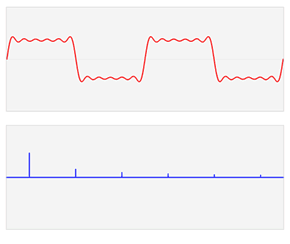
\includegraphics[width=0.5\textwidth]{assets/time-frequency.png}
	\end{figure}
		\subsubsection{Autocorrelation}
		A standard method of time-domain \f0 detection is autocorrelation. It exploits the fact that a periodic or quasiperiodic waveform such as a sustained sung note will be self-similar by the definition of periodicity. If we compare a waveform with a copy of that waveform offset by the period of the waveform i.e. \(\f0 ^{-1}\) then we should expect to see a strong correlation between them. So autocorrelation works by iterating over all the possible offset values, and determining which one has the best correlation. This correlation value for each different offset is described by the equation below, where x is the signal function, N is the window size of the waveform you are considering, and v is the offset value.  \[R_x(v) = \sum_{n=0}^{N-1-v} x[n]x[n+v]\]
		\subsubsection{Limitations}
		One fundamental limitation of Autocorrelation is that octave errors are frequently encountered. This occurs when the offset is calculated to be double what it should be, and is prone to happening as the nature of a periodic wave is such that if you shift it along twice the offset then you will also end up with a valid offset.
	
\section{Audio processing}
